\subsection{Implementation}\label{conflict_implementation}
In this section, we explain the objective and scope of the implementation, the functionality and the programming languages used.

The entire implementation is available in the GitHub repository \footnote{https://github.com/amirrabieyannejad/conflict\_analysis\_between\_USs/tree/main}.
\subsubsection*{Methodology}
This section explains and introduces tools that are required during the development process.

Following approach and tools are necessary in order to develop our workflow:
\begin{itemize}	
	\item Java as programming language\footnote{https://www.java.com/de/}: Java is a widely used object-oriented programming language.
	
	\item GitHub as version control\footnote{https://github.com/}: GitHub is a developer platform that allows developers to create, store, manage and share their code. It uses Git software, providing the distributed version control of Git plus access control, bug tracking, software feature requests, task management, continuous integration, and wikis for every project.
\end{itemize} 
\subsubsection*{Implementation Phases}\label{conflict_phases}
This section contains a step-by-step guide to implementation, starting with the set-up and ending with the extracting report.

Following steps implies the classes and methods related to org.backlogconflict.code.preparation:
\subsubsection*{Extracting Parts of USs from the Input Dataset}\label{conflict_step_json_transformer}
In this section, we explain the methods we used to convert the US data structured in JSON files into a custom US data structure that splits the elements such as Entity, Action, Contain, Target in terms of their occurrence in the main and benefit part. 
\subsubsection*{Methods of the USPartExtractor Class}
In this section, the methods of the USPartExtractor class is described as follows:
\begin{itemize}
	
	\item getStringFromOffset: This method was designed to extract a substring from a given main text of US based on the start and end offsets.
	
	As input it receives the text of US, a start offset and an end offset as an integer and as output it extracts the part of the text of US that starts at "start offset" and ends just before "end offset".
	
	\item runUSPartExtractor: This method processes multiple datasets by reading JSON lines from input files, transforming each JSON object, and then writing the transformed JSON objects to output files.
	
	As input it receives:
	\begin{itemize}
		\item An array of dataset names: each name in the array corresponds to a specific dataset that is processed
		
		\item The base directory path in which the dataset files are located. This path is used to construct the full file paths for reading inputs and writing outputs.
	\end{itemize}	
	It iterates through each dataset name in the "dataSets" array and constructs the paths of the input and output file based on the dataset name of the "filePath".
	
	It also reads all lines from the input file and passes them to the \texttt{transformJson} method for the transformation process. Finally, it writes the result to the output file.
	
	\item transformJson: This method is the main component of the USPartExtractor class. It processes a JSON object that represents a US, extracts and categorises its entities and relationships according to their occurrence in the main or benefit part of the US text and assigns this information in a new JSON structure.
	
	As input it receive the original JSON object containing information about a US, including text, entities, and relations.
	
	In this method following steps were carried out:
	\begin{itemize}
		\item It initialize a JSON object to hold the transformation data and extract the basic information like "Text" and "ID" of US as well as "PID"(project ID)
		
		\item It initialises two JSON objects, namely \texttt{Main} and \texttt{Benefit}, and specifies the elements and their relationships accordingly.
		
		\item It initialises JSON arrays for various elements such as "Persona", "Entity", "Action" and splits them based on the start and end offsets of the benefit part into "Main" or "Benefit" JSON object.
		
		If the end offset of an element is smaller than the start offset of the benefit string, it is considered to be an element of the main part, otherwise it is considered to be an element of the benefit part.
		
		\item Iterates through each relation and determines the elements involved. If both elements belong to the main part, a relation is initialised in the "Main" JSON object according to their category (Triggers, Targets, or Contains). 
		
		If both elements belong to the benefit part, a relation is initialised in the "Benefit" JSON object according to their category (Triggers, Targets, or Contains). 
		
		If elements belong to different parts of US, the relation is initialised in a \texttt{Mix} JSON object.
		
	\end{itemize}
	As output a JSON object containing the transformed data will be returned.
\end{itemize}
\subsubsection*{Addition of Action Annotations into Dataset}\label{conflict_action_annotation}
In this section, we explain the classes and their methods that we used to retrieve action annotations associated with the verb from the action annotation database using \textit{VerbFinder} class. Finally, we insert the retrieved action annotations into the JSON structure of the US using \textit{ActionsAnnotationsCreator} class.
\subsubsection*{Methods of the VerbFinder Class}
In this section, the methods of the VerbFinder class is described as follows:
\begin{itemize}	
	\item loadCSV: This method reads a CSV file with verb and action annotation pairs, processes each line and fills a map with these pairs so that when the VerbFinder class is initialised, a map with verb and action annotation pairs is available to retrieve the action annotations as needed.
	
	It receives a file path of the CSV file to be read as input. The method does not return a value directly.
	
	\item getActionAnnotations: This method retrieves the action annotations associated with a specific verb from a pre- populated map (verbMap).
	
	As input, it receives a verb as a string for which the action annotations are to be retrieved.
	
	The method then accesses the verbMap and uses the verb provided as a key.
	
	As output, it receives the corresponding action annotation from the map. If the verb is not available in the verbMap, the method returns \texttt{null}.
	
\end{itemize}
\subsubsection*{Methods of the ActionsAnnotationsCreator Class}
In this section, the methods of the ActionsAnnotationsCreator class is described as follows:
\begin{itemize}	
	\item addActionsAnnotations: This method reads JSON files for each dataset, initialize the VerbFinder with provided file path, adds action annotations to each JSON object correspond to specific US within these files, and saves the modified JSON objects back to the files.
	
	As input it receives:
	\begin{itemize}
		\item An array of dataset names which each name corresponds not only to a subdirectory containing a JSON file to be processed, but also to the file name. 
		
		\item The base directory path in which the dataset files are located. This path is used to construct the full file paths for reading inputs and writing outputs.
		
		\item The base directory path where the CSV file is located. This path is used to build the full file paths for reading the database with the action annotations to initialise the map(verbMap).
	\end{itemize}
	
	The method does not return any value. Instead, it modifies the JSON files in place by adding action annotations to each JSON object related to specific US in the file.
	
	\item addActionAnnotations: This method processes a JSON object that corresponds to a US in order to add action annotations to the "Targets" and "Contains" relationships within the "Main" part of the US in JSON object.
	
	As input, it receive a JSON object representing a US with nested structures for "Main" and "Benefit" part, each containing "Targets", "Contains" arrays.
	
	The method modifies the JSON object by adding the action annotations to the "Targets" and "Contains" relations within the "Main" part.
		
	\item findActionsAnnotations: This method retrieves the action annotation associated with a given verb. This method act as a utility for mapping verbs to their corresponding action annotations using the instance VerbFinder class.
	
	As input, it takes the verb for which the action annotation is to be found. The output returned is a String containing the action annotations for the verb provided.	
\end{itemize}

Figure \ref{fig:conflict_prepration_package_class_diagram} is a class diagram that illustrates the attributes, operations and relationships related to the org.backlogconflict.code.preparation package.
\begin{figure}[h]
	\centering
	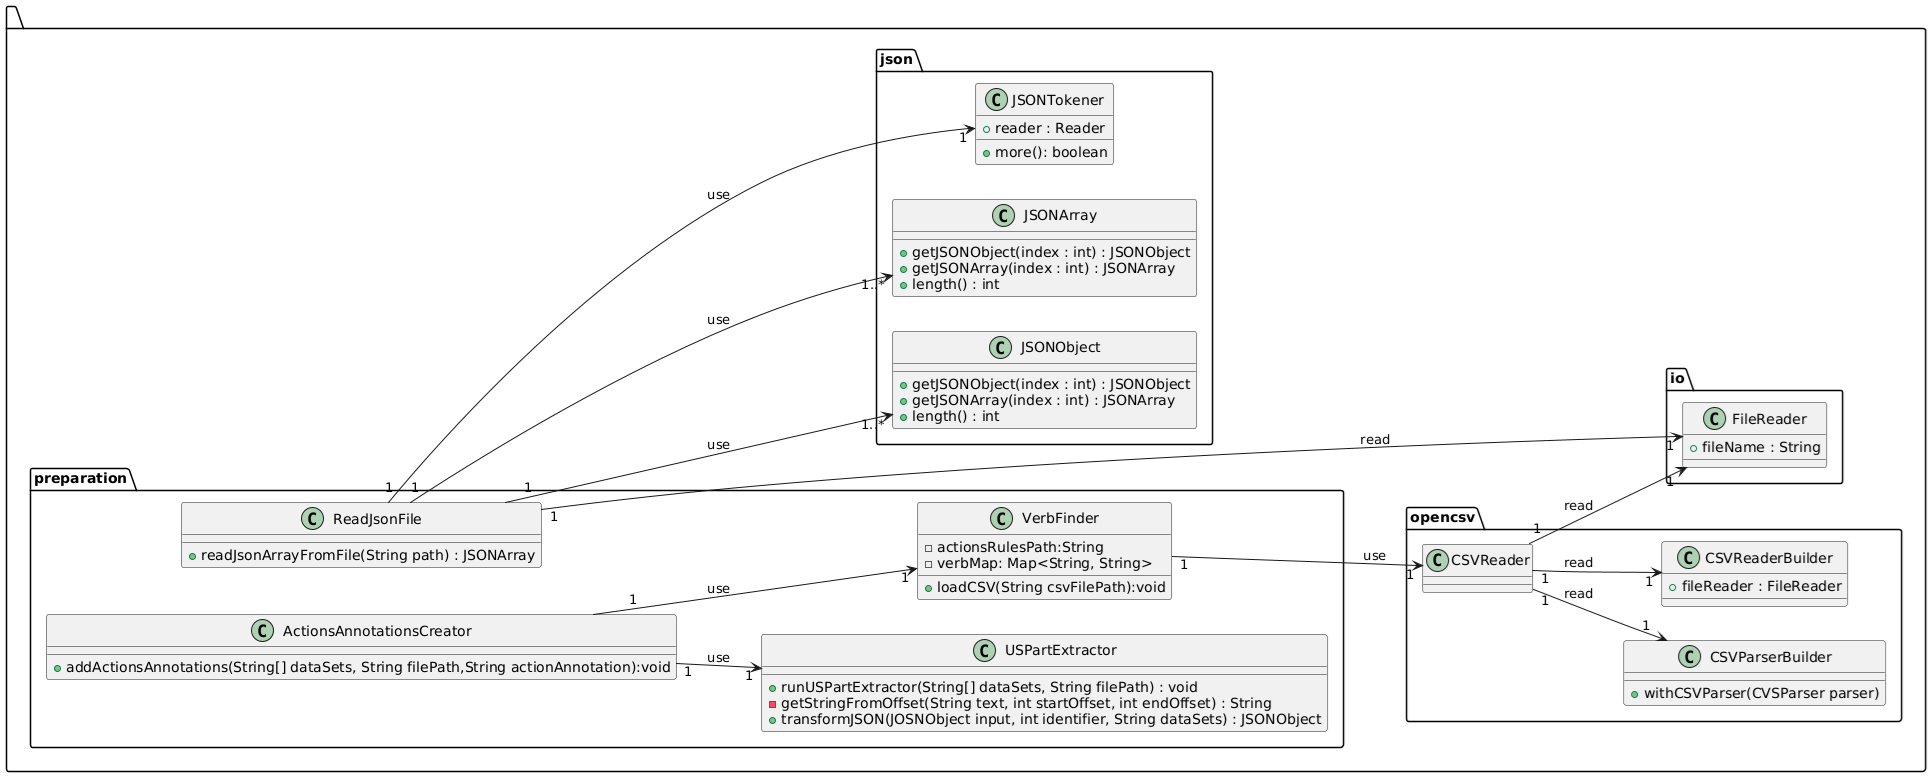
\includegraphics[scale=0.3]{conflict_prepration_package_class_diagram}
	\caption{Class diagram of the org.backlogconflict.code.preparation class and its relationships}\label{fig:conflict_prepration_package_class_diagram}
\end{figure}
\subsubsection*{Storing Conflict Pair into ConflictPair Class}
To store the elements of a conflict pair, we implement the class \textit{ConflictPair} to store the information needed to extract a textual report using \textit{ReportMaker} class.

The ConflictPair class contains the following methods that are important for the ReportMaker class:
\begin{itemize}
	\item get/setActionAnnotationUs1: The setter method stores the \textit{action annotation} for the first US in the conflict pair and the getter method retrieves it.
	
	\item get/setActionAnnotationUs2: The setter method stores the \textit{action annotation} for the second US in the conflict pair and the getter method retrieves it.
	
	\item get/setActionUs1: The setter method stores the \textit{action} for the first US in the conflict pair and the getter method retrieves it.
	
	\item get/setActionUs2: The setter method stores the \textit{action} for the second US in the conflict pair and the getter method retrieves it.
		
	\item get/setConflictReason: The setter method stores the \textit{conflict reason} of conflict pair and the getter method retrieves it.
	
	\item get/setJsonConflict1: The setter method stores the \textit{JSON object} containing all JSON elements relating to first US, and the getter method retrieves it.
	
	\item get/setJsonConflict2: The setter method stores the \textit{JSON object} containing all JSON elements relating to second US, and the getter method retrieves it.
	
	\item get/setNounContainUs2: The setter method stores the textit{contain entity} of second US, and the getter method retrieves it.
	
	\item get/setNounMainUs1: The setter method stores the textit{entity} of first US, and the getter method retrieves it.
	
	\item get/setpId: The setter method stores the \textit{P\_ID}(Project ID), and the getter method retrieves it.
	
	\item get/setUsId1: The setter method stores the \textit{US\_ID} of first US in the conflict pair, and the getter method retrieves it.
	
	\item get/setUsId2: The setter method stores the \textit{US\_ID} of second US in the conflict pair, and the getter method retrieves it.
	
	\item get/setConflictPair1: The setter method stores the \textit{US\_Nr} of first US in the conflict pair, and the getter method retrieves it.
	
	\item get/setConflictPair2: The setter method stores the \textit{US\_Nr} of second US in the conflict pair, and the getter method retrieves it.
	
	\item equals(Override): The equals method is overridden to provide a custom definition of equality for ConflictPair objects. Two ConflictPair objects are considered equals if:
	\begin{enumerate}
		\item They are the same instance.
		
		\item They are of the same class.
		
		\item Their \textit{conflictPair1} and  \textit{conflictPair2} fields are equal.
		
	\end{enumerate}
	This custom equality definition is used to compare \textit{ConflictPair} objects based on the value of \textit{conflictPair1} and \textit{conflictPair2}.

	\item hashCode(Override): This method is overridden to provide a custom hashcode calculation for ConflictPair objects. This hashcode calculation ensures that equal ConflictPair objects (as determined by the \textit{equals} method) have the same hashcode, which ensures that the behaviour of HashMap collections is correct.
	
\end{itemize}

\subsubsection*{ReportMaker Class}
To find conflict pairs and store their elements in the ConflictPair object, we must first iterate through each US and verify the US in pairs with the defined criteria. 

Figure \ref{fig:conflict_report_maker_class_diagram} is a class diagram that illustrates the attributes, operations and relationship related to the extraction of conflict pairs founded by tool and their storage in a ConflictPair object.
\begin{figure}[h]
	\centering
	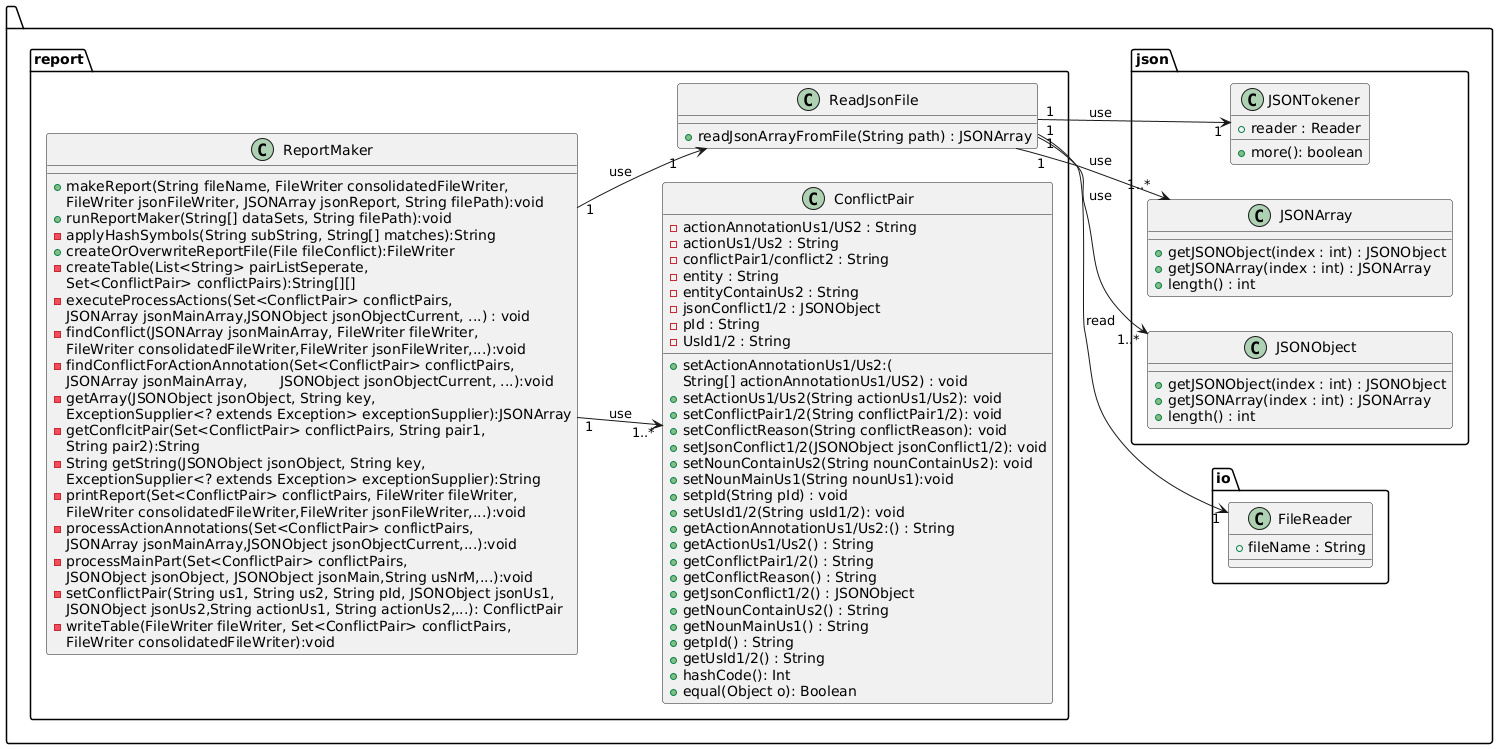
\includegraphics[scale=0.27]{conflict_report_maker_class_diagram}
	\caption{Class diagram related to \textit{org.backlogconflict.code.report} package }\label{fig:conflict_report_maker_class_diagram}
\end{figure} 

\subsubsection*{Methods related to Extracting and Reporting Conflict Pairs}
In order to report conflict pairs such with information such as highlighting USs texts with hash mark(\#), conflict pair, affected entity, contain entity related to second US, action of USs, and conflict reason, following methods in the ReprortMaker class are defined:

\begin{itemize}
	\item applyHashSymbols: This method changes a given substring by surrounding the specified matching elements with hash symbols (\#). It ensures that only the words that match the elements in the provided array are changed. 
	
	As input it receive a substring in which the matching elements will be replaced with hash-surrounded versions and an array of string representing the elements to be surrounded by hash symbols within the substring.
	
	The method returns a modified version of the substring where each specified match is surrounded by hash symbols.
	
	\item createOrOverwriteReportFile: This method is designed to create or overwrite a report file. It ensures that a FileWriter object is returned, which can then be used to write to the specified file.
	
	As input it receive file object representing the file that needs to be created or overwritten.
	
	As output, it returns a FileWriter object that is set up to write the specified file, regardless of whether it was newly created or overwritten.
	
	\item createTable: This method constructs a two-dimensional table (a matrix) that represents conflicts between pairs of USs. The header rows of the table and the first column are filled with modified identifier of USs (e.g. us\_xx instead of user\_story\_xx) from a given list and the cells in the table are filled with \texttt{X} based on the conflicts found between pairs of these USs using \textit{getConflcitPair} method.
	
	As input it receives a list of strings where each string represents a US and a set of ConflictPair objects representing conflicts between pairs of USs.
	
	As output, the method returns a two-dimensional array that represents the conflict table. The header rows and the first column are identifiers of the conflicting USs and the cells contain \texttt{X} if there is a conflict between these two USs.
	
	\item getConflcitPair: This method searches for conflicts between a pair of US-pairs and returns \texttt{X} if there is a conflict between two USs, otherwise it returns a white space.
	
	\item runReportMaker: The runReportMaker method generates conflict reports for a number of datasets using the \textit{makeReport} method. It creates both a consolidated text report and a JSON report that summarises the conflicts found in the specified datasets.
	
	As input, it receives an array with the names of the datasets to be processed and the path of the base file in which the datasets are located.
	
	As output, it produces a text file containing the consolidated conflict report and a JSON file containing the conflict report in JSON format.
	
	\item makeReport: This method generates a conflict report for a single dataset. It reads the dataset from input JSON file, processes it to find conflicts using \textit{findConflict} method, and writes the results to both a text file and a JSON report.
	
	It receives the following inputs:
	\begin{itemize}
		\item fileName: The name of the dataset file to process.
		
		\item consolidatedFileWriter: A FileWriter object to write the consolidated conflict report for all datasets.
		
		\item jsonFileWriter: A FileWriter object to write the JSON conflict report for single dataset.
		
		\item jsonReport: A JSON array object for collecting conflict reports from a dataset.
		
		\item filePath: The base file path where the dataset files are located.
		
	\end{itemize}
	As output, the method updates the consolidated conflict report file and the JSON conflict report with the conflicts found in the specified dataset.
	
	A separate conflict report text file for the individual dataset is created or overwritten with the conflict details.
	
	\item findConflict: This method analyses a given JSON array to identify and report conflicts within the USs. It iterates through each JSON object which represents the US in the array, processes the "Main" part of each JSON object, and collects conflict information using \textit{processMainPart} method. The results are then written to specified file writers and a JSON report using \textit{printReport} method.
	
	As input, the same input related to the makeReport method is passed.
	
	As output, The method populates the provided FileWriter objects and JSONArray with conflict information derived from the input JSON array. It identifies conflicts by processing the "Main" part of each JSON object and aggregates the results for reporting.
	
	\item processMainPart: This method processes the "Main" part of a given JSON object, extracting various arrays and strings using \textit{getArray} as well as getString methods. It then checks for action annotations using \textit{processActionAnnotations} method and processes them to identify conflicts. The method adds the conflicts to a provided set of conflict pairs.
	
	It receives the following inputs:
	\begin{itemize}
		\item conflictPairs: A set to store the identified conflict pairs.
		
		\item jsonObject: The JSON object currently being processed representing specified US.
		
		\item jsonMain: The "Main" part of the JSON object(related to the specified US) currently being processed.
		
		\item usNrM: The US identifier of the current JSON object.
		
		\item jsonMainArray: The main JSON array containing all the USs to be analysed.
		
		\item conflicts: A set US identifier to store unique conflict pair.
				
	\end{itemize}	
	The method does not return a value.
	
	\item processActionAnnotations: This method processes action annotations from JSON objects that refer to USs in order to process action annotations. Iterates through the element \textit{Target Action Annotations}, checks whether there are multiple action annotations and executes the associated actions to process these annotations. If an action annotation that refers to an action contains multiple actions, the \textit{executeProcessActions} method is called for each part of the annotation. Identified conflicts are added to a provided set of conflict pairs.
	
	It receives the following inputs:
	\begin{itemize}
		\item usNrM: The US identifier of the current JSON object.
		
		\item jsonObject: The JSON object currently being processed which corresponds to specified US.
		
		\item actionArray: The array of actions in the US JSON object.
		
		\item entityArray: The array of entities in the US JSON object.
		
		\item triggersArray: The array of triggers in the US JSON object.
		
		\item targetsArray: The array of targets in the US JSON object.
		
		\item containsArray: The array of contains in the US JSON object.
		
		\item text: The text associated with the US JSON object.
		
		\item persona: The array of personas in the US JSON object.
		
		\item conflicts: A set to store unique conflict strings.
	\end{itemize}
	The method does not return a value.
	
	\item executeProcessActions: This method processes specific action annotations (like preserve, delete, create, and forbid) by checking for conflicts with other annotations in the JSON data. It uses the \textit{findConflictForActionAnnotation} method to identify and handle these conflicts, adding them to a set of conflict pairs.
	
	The method uses a switch statement to process the action annotation based on the defined criteria and handle it accordingly. For each case in the switch statement, the method calls \textit{findConflictForActionAnnotation} with different parameters to identify potential conflicts based on specific criteria.
	
	It receives the following inputs:
	\begin{itemize}
		\item usNrM: The US identifier of the current JSON object.
		
		\item jsonObject: The JSON object currently being processed which corresponds to specified US.
		
		\item actionArray: The array of actions in the US JSON object.
		
		\item entityArray: The array of entities in the US JSON object.
		
		\item triggersArray: The array of triggers in the US JSON object.
		
		\item targetsArray: The array of targets in the US JSON object.
		
		\item containsArray: The array of contains in the US JSON object.
		
		\item text: The text associated with the US JSON object.
		
		\item persona: The array of personas in the US JSON object.
		
		\item conflicts: A set US identifier to store unique conflict pair.
		
		\item verb: The verb extracted from the \textit{Target Action Annotations}.
		
		\item noun: The noun extracted from the \textit{Target Action Annotations}.
		
		\item actionAnnotation: The action annotation (e.g., "preserve", "delete").
		
		\item nounMainUs1: The entity of first US.
	\end{itemize}
	The method does not return a value.
	
	\item findConflictForActionAnnotation: This method is responsible for identifying conflicts between USs based on certain action annotations and entity relationships within a JSON dataset. Iterates through all JSON objects in a dataset to compare the current US with others. It iterates through "Target Action Annotations" to compare action annotations and entities. It also iterates through the "Contain Action Annotations" array to compare the contained entities. If a conflict is detected between two US, the \textit{setConflictPair} method is used to create a ConflictPair object with specific information and add the conflictPair object to a set called \textit{conflictPairs}.
	
	It receives the following inputs:
	\begin{itemize}
		
		\item conflictPairs: A set to store identified conflict pairs.
		 
		\item jsonMainArray: The main JSON array containing all the USs to be analysed.
		
		\item jsonObjectCurrent: The current US JSON object being processed.
		
		\item actionAnnotationUs1: The action annotation from the first US.
		
		\item criticalActionAnnotation: The critical action annotation that triggers conflicts.
		
		\item entityUs1: The entity associated with the first US.
		
		\item actionUs1: The action associated with the first US.
		
		\item conflicts: A set US identifier to store unique conflict pair.		
		
	\end{itemize}
	The method does not return a value.
	
	\item setConflictPair: This method effectively initializes and populates a \textit{ConflictPair} object with the provided parameters, encapsulating all necessary information about a conflict pair between two USs.
	
	It receives the following inputs:
	\begin{itemize}
		\item us1, us2: Identifiers for the conflicting USs.
		
		\item pId: Project ID associated with the USs.
		
		\item jsonUs1, jsonUs2: JSON objects representing the conflicting USs.
		
		\item actionUs1, actionUs2: Actions associated with the conflicting USs.
		
		\item actionAnnotationUs1, actionAnnotationUs2: Action annotations related to the conflicting actions.
		
		\item conflictReason: Reason of the conflict.
		
		\item nounMainUs1: Noun associated with the first US.
		
		\item nounContainUs2: Noun contained within the second US, if applicable.
		
		\item usId1, usId2: User story IDs associated with first and second USs, respectively.
	\end{itemize}
	As output, it returns the populated ConflictPair object to the caller. 
	
	\item getArray: This method is designed to retrieve a JSON array from a JSON object based on a specified key.
	
	It receives the following inputs:
	\begin{itemize}
		\item jsonObject: The JSON object to retrieve the JSON array.
		
		\item key: The key whose associated JSON array is to be retrieved from JSON object.
		
		\item exceptionSupplier: A functional interface that can supply an exception of a specific type if needed. This is used to handle cases where the expected key is not found in the JSON object.
		
	\end{itemize}
	If the key exists in the JSON object, the corresponding JSON array is retrieved as output, otherwise an exception is thrown.
	
	\item getString: This method is designed to retrieve a String from a JSON object based on a specified key.
	
	It receives the following inputs:
	\begin{itemize}
		\item jsonObject: The JSON object to retrieve the string.
		
		\item key: The key whose associated string is to be retrieved from JSON object.
		
		\item exceptionSupplier: A functional interface that can supply an exception of a specific type if needed. This is used to handle cases where the expected key is not found in the JSON object.
		
	\end{itemize}
	If the key exists in the JSON object, the corresponding string is retrieved as output, otherwise an exception is thrown.
	
	\item printReport: This method is responsible for creating a textual, tabular and JSON report based on the conflict pairs found during processing. For each ConflictPair, it extracts detailed information such as IDs, text of the USs, actions, annotations, conflict reasons, highlighting of the affected elements in the texts of the USs in the main parts using the \textit{applyHashSymbols} method. 
	
	It receive following inputs: 
	\begin{itemize}
		\item conflictPairs: A set of ConflictPair objects.
		
		\item fileWriter, consolidatedFileWriter, jsonFileWriter: These are FileWriter objects responsible for writing text and JSON data to respective files.
		
		\item fileName: A String representing the name of the dataset being processed.
	\end{itemize}
	The method does not return a value.
	\end{itemize}
	
\subsubsection*{Import Result for Evaluation}
In this step, we collect all potential conflicts found in an Excel file called ‘Conflict\_Evaluation’ by creating a report in JSON format and using the following VBA script\footnote{https://github.com/amirrabieyannejad/conflict\_analysis\_between\_USs/blob/main/ 00\_annotated\_datasets/extractFromJSONFiles\_Version(new).xlsm} to import the required information into the Excel file:
Listing \ref{list:conflict_vba} illustrates the implemented VBA script that uses the JSON report to import the required information into an Excel file.
\begin{MyListing}
	\paragraph{}
	\centering
	%\lstinputlisting[basicstyle=\ttfamily\footnotesize]{Listing/TextualReportSample.txt}
	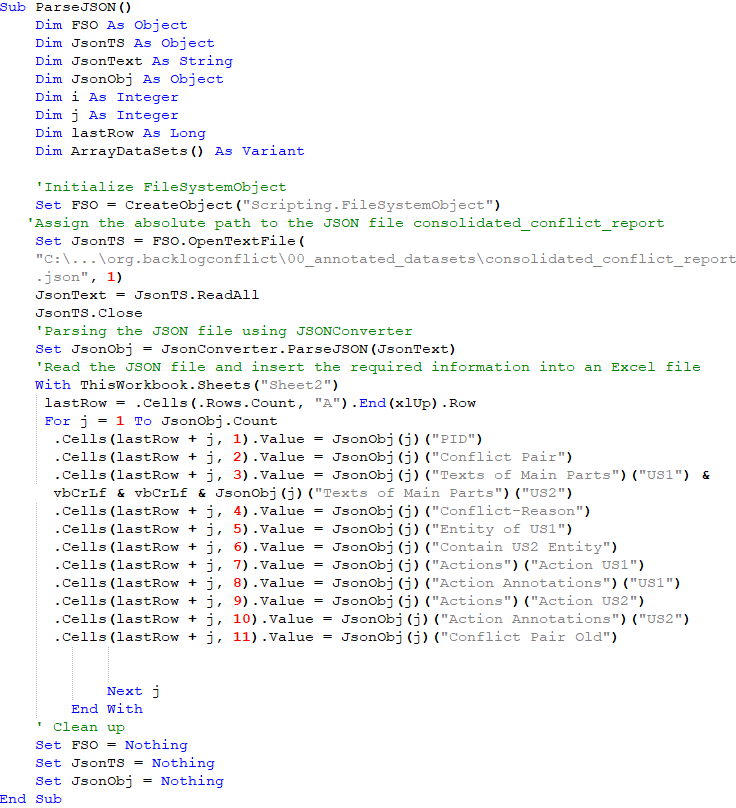
\includegraphics[scale=0.7]{Listing/conflict_vba.png}
	\caption{VBA script for importing information from a JSON report into an Excel file}\label{list:conflict_vba}
\end{MyListing}	
\subsubsection*{Error Handling}
There were erroneous data in the datasets forcing us to handle them correctly. Therefore, we implement/use the following exceptions to accurately distinguish and handle them.

The following classes, which extend the \textit{Exception} class, are used in \textit{org.backlogconflict. code.preparation} and \textit{org.backlogconflict. code.report} packages:
\begin{itemize}
	\item MainPartInJsonFileNotFound: Is triggered if the JSON object "Main" could not be found in the US JSON object.
	
	\item ActionAnnotationInJsonFileNotFound: Is triggered if the entry \textit{Action Annotations}, which contains \textit{Targets/Contains Action Annotations}, is not present in the US JSON object and its absence should be reported.
	
	\item ActionInJsonFileNotFound: Is triggered if the entry \textit{Action} is not present in the US JSON object and its absence should be reported.
		
	\item ContainsInJsonFileNotFound: Is triggered if the entry in \textit{Contains} is not present in the US JSON object and its absence should be reported.
	
	\item EntityInJsonFileNotFound: Is triggered if the entry \textit{Entity} is not present in the US JSON object and its absence should be reported.
	
	\item PersonaInJsonFileNotFound: Is triggered if the entry \textit{Persona} does not exist in the US JSON object for a specified US.
	
	\item TextInJsonFileNotFound: Is triggered if the entry \textit{Text} does not exist in the US JSON object for a specified US. 
	
	\item UsNrInJsonFileNotFound: Is triggered if the entry \textit{Us\_Nr} does not exist in the US JSON object for a specified US.
	
	\item TargetsInJsonFileNotFound: Is triggered if the entry \textit{Targets} does not exist in the US JSON object for a specified US.
	
	\item TriggersInJsonFileNotFound: Is triggered if the entry \textit{Triggers} does not exist in the US JSON object for a specific US.
	
	\item EmptyOrNotExistJsonFile: Is triggered if the JSON file is empty or does not exist.
	
	\item EntityInRelationsNotFound: Is triggered if the entity as part of \textit{relation} JSON array is not present in the US JSON object and its absence should be reported.
	
\end{itemize}
%TODO: 
%\subsubsection*{Limitations}
% 1- This tool is only suitable for the specific JSON format

% 2- As the conflict in the benefit part is not taken into account in our approach, we exclude the elements that originate from the benefit and the mix part.

% 3- The verbs are not change to root, during annotating verbs the actual verb from datasets are direktly handed over into action annotation DB.

% 3- 
\subsection{Test}\label{conflict_test}
Our objectives in this section include validating certain functions, checking the system requirements and ensuring the reliability and robustness of the implemented classes and methods.

As part of our testing strategy, we perform unit tests with \textit{JUnit} version 4\footnote{https://junit.org/junit4/}, which we selected for its compatibility with Eclipse version 2023-03. 

EclEmma\footnote{https://www.eclemma.org/} We have integrated a code coverage tool into the Eclipse IDE to ensure thorough testing and coverage. With the help of EclEmma, we systematically measured the effectiveness of our test suites and determined the test coverage for each individual class.
\subsubsection*{Configuration of Test Environment}
In the main project \textit{org.backlog}, we create a separate package called \textit{org.backlogconflict.test}. This package contains the following Java classes, which correspond to the respective Java source code files:
\begin{itemize}
	
	\item USPartExtractorTest
	
	\item ActionsAnnotationsCreatorTest
	
	\item VerbFinderTest
	
	\item ReportMakerTest
	
\end{itemize}
\subsubsection*{Scope of Testing}
The scope of the tests depends on the system requirements and the implemented classes and their methods. The implemented error handling classes are also tested.
\subsubsection*{Test Cases and their Code Coverage}
We describe the individual test cases that are carried out during the test process. Each test case contains a description of the test scenario, the data provided and the expected result. To refine and improve our test cases, we used a code coverage report created by EclEmma to increase coverage and ensure a more reliable, error-resistant application.

Table \ref{tb:test_cases_json_transformer} shows the test cases for the USPartExtractor.java class and Figure \ref{fig:code_coverage_json_transformer} shows the code coverage.

%\newgeometry{margin=2.5cm}
%\begin{landscape}
\thispagestyle{empty}
%\begin{figure}[h]
\begingroup
\centering
\scriptsize
\renewcommand{\arraystretch}{1,5}
\keepXColumns
	\begin{tabularx}{\textwidth}{X  X  X  X}
	\hline
	Test Case &Supplied Data&Expected Outcome&Description\\
	\hline\hline
	\endfirsthead
	\hline
	Test Case &Supplied Data&Expected Outcome&Description\\
	\hline\hline
	\endhead
		BenefitNotExist&Assign USs without benefit part&The length of the entries(action, entity, contains, targets) for the benefit should be null&Check what happens if the US has no benefit part\\
		
		EntityInRelationNotFound \newline(Case1)&Preparing a JSON object whose entity entry is not defined as an entity in the relation entries assigned as the first reference&Through an exception: \textit{NullPointerException}&Checks whether the first referencing entity is already defined as an entity in the relation entries\\
		
		
		EntityInRelationNotFound \newline(Case2)&Preparing a JSON object whose entity entry is not defined as an entity in the relation entries assigned as the second reference&Through an exception: \textit{NullPointerException}&Checks whether the second referencing entity is already defined as an entity in the relation entries\\
		
		EmptyOrNotExistJsonFile&Assign an empty JSON file&Through an exception: \textit{NoSuchFileException}&Checks whether the JSON file is empty\\
		
		testPid&JSON file with the project ID&Create JSON object "PID" which contain the project ID of US&Checks whether the project ID was created as expected\\
		
		UnexpectedType&JSON file with a US with unexpected type&Through an exception: \textit{JSONException}&Checks whether the expected types (action, entity, text, etc.) in the corresponding US pass on in the JSON file and not unexpected\\
		
		
		\hline
		\caption{Test cases for USPartExtractor  class}\label{tb:test_cases_json_transformer}
	\end{tabularx}
	%\captionof{table}{Test cases for RuleCreator  class}\label{tb:test_cases_rule_creator}
\endgroup

\begin{figure}[h]
	\centering
	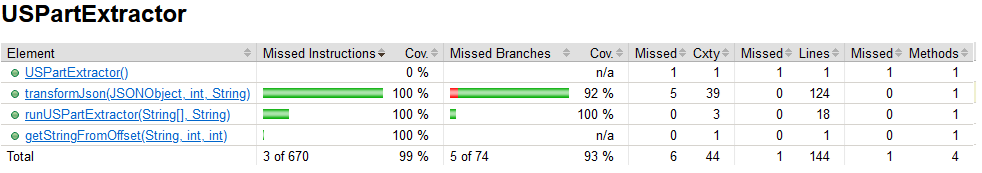
\includegraphics[scale=0.5]{code_coverage_json_transformer}
	%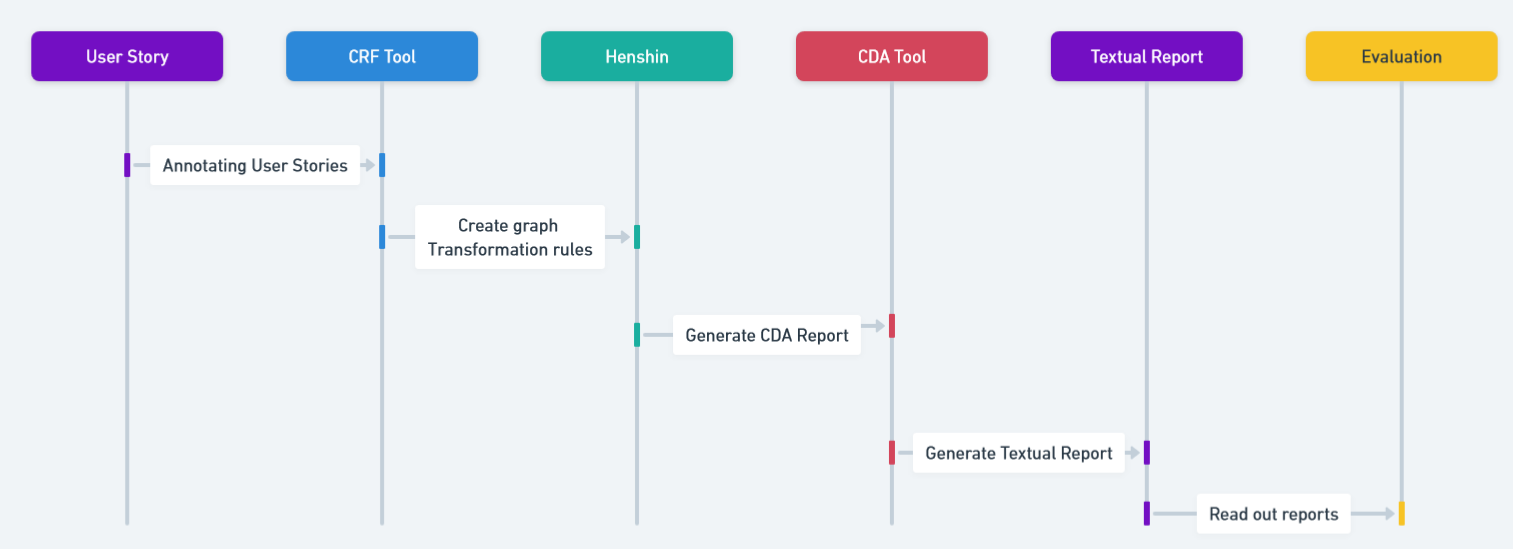
\includegraphics[scale=0.35]{sequence_diagram}
	\caption{Code coverage related to class USPartExtractor}\label{fig:code_coverage_json_transformer}
\end{figure} 


Table \ref{tb:test_cases_verb_finder} shows the test cases for the VerbFinder.java class and Figure \ref{fig:code_coverage_verb_finder} shows the code coverage.

%\end{figure}
%\end{landscape}
%\restoregeometry
%\newgeometry{margin=2.5cm}
%\begin{landscape}
	\thispagestyle{empty}
%	\begin{figure}[h]
		\begingroup
		\centering
		\scriptsize
		\renewcommand{\arraystretch}{1,5} 
		\keepXColumns
		\begin{tabularx}{\textwidth}{X  X  X  X}		
			\hline
			Test Case &Supplied Data&Expected Outcome&Description\\
			\hline\hline
			\endfirsthead
			\hline
			Test Case &Supplied Data&Expected Outcome&Description\\
			\hline\hline
			\endhead
			testLoadCSV\linebreak (Case1)&Assign a CSV file that contains two columns: one for verbs and one for action comments, so that both columns contain no empty cells&Action Annotation corresponds to verbs should be returned&Checks whether the action note has been returned accordingly in respect of the verb\\
			
			testLoadCSV\linebreak (Case2)&Assign a CSV file that contains two columns: one for verbs and one for action comments, so that one column contain empty cell&A verb without an assigned action annotation should be ignored&Checks whether the action annotation has been returned accordingly in respect of the verb\\
			\hline
				\caption{Test cases for VerbFinder class}\label{tb:test_cases_verb_finder}
		\end{tabularx}		
	%	\captionof{table}{Test cases for ReportExtractor  class}\label{tb:test_cases_report_extractor}
		\endgroup
	%\end{figure}

\begin{figure}[h]
	\centering
	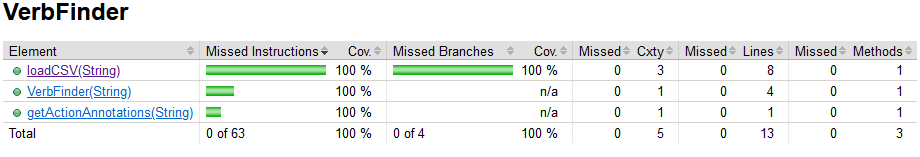
\includegraphics[scale=0.5]{code_coverage_verb_finder}
	\caption{Code coverage related to class VerbFinder}\label{fig:code_coverage_verb_finder}
\end{figure} 

Table \ref{tb:test_cases_actions_annotations_creator} shows the test cases for the ActionsAnnotationsCreator.java class and Figure \ref{fig:code_coverage_actions_annotations_creator} shows the code coverage.

%\end{figure}
%\end{landscape}
%\restoregeometry
%\newgeometry{margin=2.5cm}
%\begin{landscape}
\thispagestyle{empty}
%	\begin{figure}[h]
	\begingroup
	\centering
	\scriptsize
	\renewcommand{\arraystretch}{1,5} 
	\keepXColumns
	\begin{tabularx}{\textwidth}{X  X  X  X}		
		\hline
		Test Case &Supplied Data&Expected Outcome&Description\\
		\hline\hline
		\endfirsthead
		\hline
		Test Case &Supplied Data&Expected Outcome&Description\\
		\hline\hline
		\endhead
		ActionsAnnotationsCreator&Assign a JSON file without entries of action annotations (target or contains action annotation)&Create action annotation related to target action annotated&Checks whether the JSON array for the corresponding action has been created for the target\\
		
		
		\hline
		\caption{Test cases for ActionsAnnotationsCreator class}\label{tb:test_cases_actions_annotations_creator}
	\end{tabularx}		
	%	\captionof{table}{Test cases for ReportExtractor  class}\label{tb:test_cases_report_extractor}
	\endgroup
	%\end{figure}
	
	\begin{figure}[h]
		\centering
		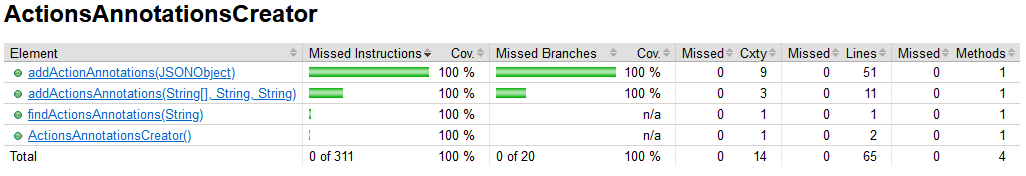
\includegraphics[scale=0.5]{code_coverage_actions_annotations_creator}
		\caption{Code coverage related to class ActionsAnnotationsCreator}\label{fig:code_coverage_actions_annotations_creator}
	\end{figure} 
	
Table \ref{tb:test_cases_report_maker} shows the test cases for the Evaluation.java class and Figure \ref{fig:code_coverage_report_maker} shows the code coverage.

%\newgeometry{margin=2.5cm}
%\begin{landscape}
%\thispagestyle{empty}
%\begin{figure}[h]
\begingroup
\centering
\scriptsize
\renewcommand{\arraystretch}{1,5} 
\keepXColumns

\begin{tabularx}{\textwidth}{X  X  X  X}
	\hline
	Test Case &Supplied Data&Expected Outcome&Description\\
	\hline\hline
	\endfirsthead
	\hline
	Test Case &Supplied Data&Expected Outcome&Description\\
	\hline\hline
	\endhead
	
	ActionAnnotation\newline InJsonFileNotFound&Provision of a JSON object without action annotation&Through an exception:\textit{ActionAnnotation InJsonFileNotFound}&Checks whether the JSON object provided contains an entry for action annotations\\
	
	TargetActionAnnotation\newline InJsonFileNotFound&Provision of a JSON object without target action annotation&Through an exception:\textit{ActionAnnotation InJsonFileNotFound}&Checks whether the JSON object provided has an entry for target action annotations\\
	
	ContainActionAnnotation\newline InJsonFileNotFound&Provision of a JSON object without contain action annotation&Through an exception:\textit{ActionAnnotation InJsonFileNotFound}&Checks whether the JSON object provided has an entry for contain action annotations\\
	
	EntityContainExist&Provision of a conflict pair with indirect conflict through contain relation&The US-pairs should be reported as a conflict pair&Checks whether the conflict is recognised if the entity from Us belongs to contain relation\\
	
	JsonArrayNotFound&Provision of a JSON file in which a JSON array is missing&Null should be return&Checks whether the specific JSON array was not found, if so, return null\\
	
	JsonObjectNotFound&Provision of a JSON file in which a JSON object is missing&Null should be return&Checks whether the specific JSON object was not found, if so, return null\\
	
	runReportMaker\_Main&Provision of two USs that contradict each other&The conflict pair should be reported in text form&Checks whether two USs that contradict each other have already been reported as conflict pair\\
	
	MainIsEmpty&Provision of a JSON object with empty main part entry&Through an exception:\textit{MainPartInJsonFile NotFound }&Checks whether the main part entry in provided JSON object is not empty\\
	
	MainNotExist&Provision of a JSON object without main part entry&Through an exception:\textit{MainPartInJsonFile NotFound }&Checks whether the JSON object provided has main part entry\\
	
	runReportMaker\_NoConflict&Provision of a set of USs that not contradict each other&The conflict pair should not be reported&Checks whether two USs that do not contradict each other should not be reported as a conflict pair\\
	
	UsNrInJsonFileNotFound&Provision of a JSON object that don't have US identifier&Through an exception:\textit{UsNrInJsonFileNotFound}&Checks whether the JSON object in the JSON file already has an identifier\\
	
	writeTable&Provision of a conflict pair that should be reported&Conflict pair should be listed in tabular form&Check whether the conflict pair is already listed in the table\\
	\hline
	\caption{Test cases for ReportMaker  class}\label{tb:test_cases_report_maker}
\end{tabularx}

%\captionof{table}{Test cases for RuleCreator  class}\label{tb:test_cases_rule_creator}
\endgroup
\thispagestyle{empty}
%\end{landscape}
%\restoregeometry

\begin{figure}[h]
	\centering
	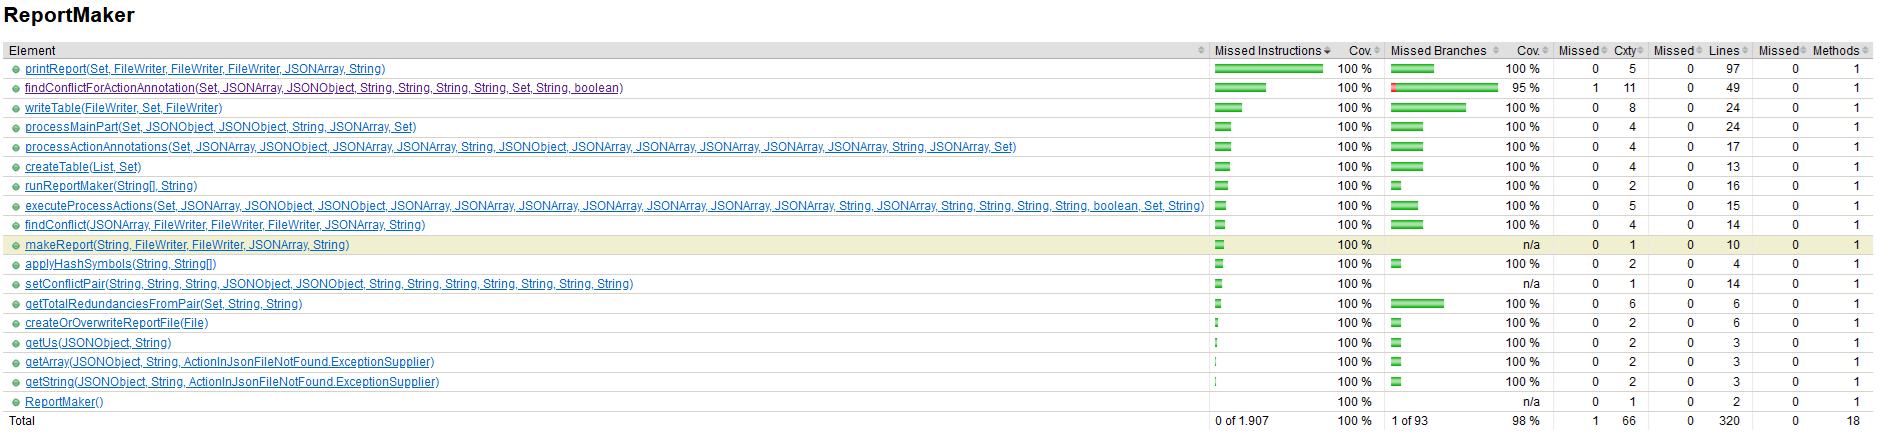
\includegraphics[scale=0.3]{code_coverage_report_maker}
	%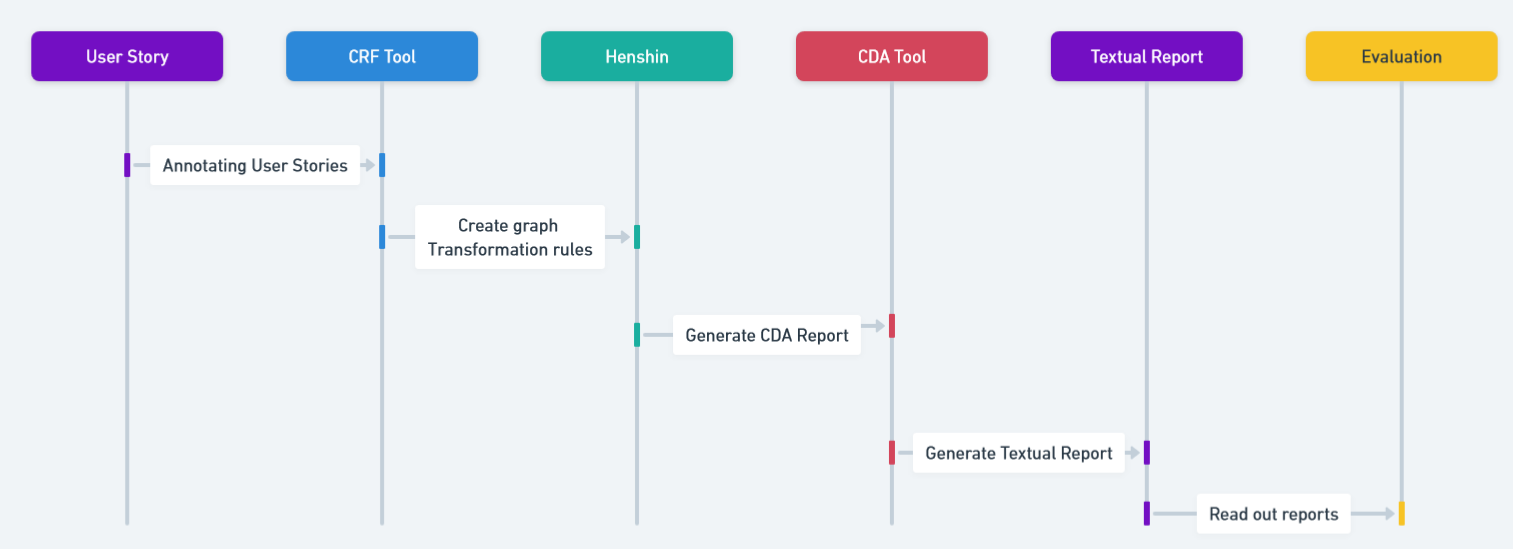
\includegraphics[scale=0.35]{sequence_diagram}
	\caption{Code coverage related to class ReportMaker}\label{fig:code_coverage_report_maker}
\end{figure}
%\subsubsection*{Performance Test}
%In this section, we describe the performance testing approach used for this project, including the test setup, key metrics, and the results of the tests.

\subsection{Evaluation}\label{conflict_evaluation}
In this section, we address two research questions (RQs) and explain how we designed and conducted the experiments for each question. We then analyse the results to answer these RQs, discuss their significance and share the findings from the results.
\subsubsection*{Research Questions}
The RQs addressed in this section are as follows:
\begin{itemize}
	\item \textbf{RQ 1}: Does our tool consistently identify conflicts between USs?
	\item \textbf{RQ 2}: How does the performance of the tool change as the count of USs in a backlog increases?
	\end{itemize}
\subsubsection*{Methodology}
To answer the RQ1, "Does our tool consistently detect conflicts between USs?", we recapitulate the methodology used to analyse conflicts between USs. We used a systematic approach that includes several important steps:
\begin{itemize}
	
	\item Data Collection: For a comprehensive assessment, we applied our approach to 19 backlog datasets presented by Mosser et al. \footnote{\href{https://github.com/ace-design/nlp-stories}{https://github.com/ace-design/nlp-stories}}. They applied the Doccano approach to these publicly available requirements datasets \cite{requirementsdatasets}.
	
	 It is also worth noting that some backlog datasets (g02, g13, g17, g27) did not follow the expected sentence structure, so we did not include them in the evaluation results to avoid unexpected behaviour. Table \ref{tb:conflcit_backlogs} shows the project number of each dataset and the count of USs.
	 
	 %empty line here
	\begingroup
	\centering
	\scriptsize
	\renewcommand{\arraystretch}{1.5} 
	\begin{tabularx}{\linewidth}{l|XXXXXXXXXXXXXXXXXXX X}
		Item&	1&	2&	3&	4&	5&	6&	7&	8&	9&	10&	11&	12&	13&	14&	15&	16&	17&	18&	19&	\\
		\hline
		Project Nr.&	g03	&g04	&g05	&g08	&g10	&g11	&g12	&g14	&g16	&g18	&g19	&g21	&g22	&g23	&g24	&g25	&g26	&g27	&g28	&Total USs\\
		\hline
		Total USs&	57&	51	&53	&66	&97	&73	&54	&67	&66	&102	&137	&69	&83	&56	&53	&100	&100	&114	&60	&1458 \\
		\caption{Project number and count of USs contained in each backlog dataset}\label{tb:conflcit_backlogs}
	\end{tabularx}	
	\endgroup
	\item Splitting the elements of the US into main and benefit parts: each element of the US (action, entity and relations) was split into main or benefit part, where the main part represents the core functionality and the benefit part describes the value for the persona. In this analysis, we only consider the conflicts between the main parts of the USs.
	
	\item Recognition of conflicts: Detection of conflicts between USs in main parts of the USs based on defined criteria.
	
\end{itemize}
\subsubsection*{Ground Truth}
To answer the first research question (RQ), our automated system needs a reference point to measure its accuracy. This reference point, called "ground truth", comes from a personal judgement and serves as a benchmark for evaluating the tool's performance.

Unlike the tool evaluation, we did not assess conflicts based on defined criteria. Instead, in the ground truth evaluation, we examined conflicts based on the text of the US-pairs detected by tool. This involved reading the text of the USs and evaluating conflicts between US-pairs in a semantic manner.

The ground truth serves as the final assessment against which the automated results are compared. It results from the personal judgement of a subject matter expert (in this case me) using a combination of expertise and experience. This personal judgement is intended to provide a reliable and accurate reference for identifying conflicts between USs.\\\\
Table \ref{tb:conflict_ground_truth} shows the summary of conflicting US-pairs as ground truth.
\begin{figure}[h]
	\begingroup
	\scriptsize
	\centering
	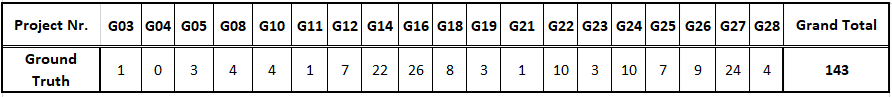
\includegraphics[scale=0.6]{Table/conflict_ground_truth.png}
	\captionof{table}{Details of the count of correctly recognised and validated conflicting US-pairs by the tool as ground truth}\label{tb:conflict_ground_truth}	
	\endgroup
\end{figure}
\subsubsection*{Evaluating Tool-Detected Conflicts Using Ground Truth}
The automated tool was developed to recognise conflicts between USs based on predefined criteria. It analyses the structure of USs to identify discrepancies that could indicate a conflict.

In contrast to ground truth, which is based on the semantic comparison of texts in the main parts of USs, the evaluation of the tool relies heavily on specified labelling (targets, triggers, contains) using the Doccano tool and predefined criteria.

Table \ref{tb:tool} shows the aggregation of the conflicting US-pairs found in the main parts evaluated by the tool.
\begin{figure}[h]
	\begingroup
	\scriptsize
	\centering
	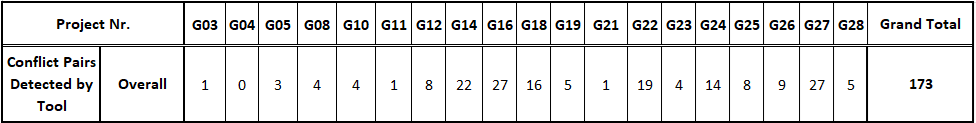
\includegraphics[scale=0.55]{Table/conflict_tool.png}
	\captionof{table}{Overall count of conflicting US-pairs in relation to the main parts assessed by the tool}\label{tb:conflict_tool}
	\endgroup
\end{figure}
\paragraph{Assessment of Result: High-Level Overview}When comparing the results provided by the tools with the ground truth, we found that 143 cases were correctly assessed as conflicting US-pairs and 30 cases were invalid on the basis of the ground truth.

Table \ref{tb:conflict_difference} shows the count of valid and invalid conflicting US-pairs assessed by the ground truth and recognised by the tool.

Based on the datasets provided, 173 conflicting US-pairs were found across all projects, with the highest count found in the backlog G27 dataset (24 cases), indicating a significant occurrence of conflicts in the USs of this project.
\begin{figure}[h]
	\begingroup
	\scriptsize
	\centering
	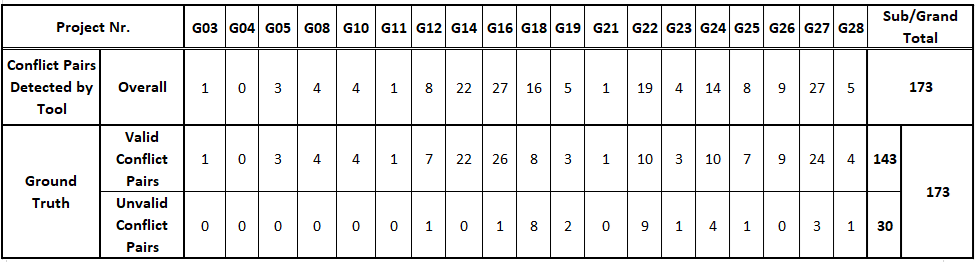
\includegraphics[scale=0.55]{Table/conflict_difference.png}
	\captionof{table}{Information on the number of discrepancies between the result provided by the tool and the ground truth}\label{tb:conflict_difference}
	
	\endgroup
\end{figure}
\paragraph{Assessment of Result: Detailed Insights}In the USs of the datasets, there are some verbs such as "have", "know" and nouns such as "data", "resource", "collection", "list", and "file" that are cross-contextual, so they do not contain generic information, which has a very negative impact on conflicts analysis (30 cases are false positives).

\begin{example}
	For example, user\_story\_983 and user\_story\_989 are reported as a conflicting US-pair in the G24 backlog dataset:\\
	\textit{user\_story\_1365:} \#G24\# As a depositor, I want to store and manage \#datasets\# via a simple web interface.\\
	\textit{user\_story\_1409:} \#G24\# As a research information manager, I want to have \#datasets\# linked to metadata about projects.\\
	The depositor needs a simple interface for uploading and managing datasets. The research information manager needs to be able to link these datasets to comprehensive metadata about the projects.\\
	These needs are not inherently conflicting, but they require careful design consideration to ensure that both needs are met effectively.\\
	To avoid the conflict, the verb "have" related to "user\_story\_1409" should be defined more precisely. The US should be amended as follows:\\
	\textit{user\_story\_1409:} \#G24\# As research information manager, I want to \textit{\texttt{link} \texttt{datasets}} to metadata about projects.\\
\end{example}

There are also annotated USs with inaccurate labelling by the Doccano tool. In other words, there is more information about the resource in concern provided in US, which leads to inconsistencies and bias.
\begin{example}
	In the dadaset of backlog G25, for example, we have a US-pair that are marked as conflict:\\
	\textit{user\_story\_1506}: \enquote{\#G25\# As a DAMS manager, I want to know when the \#application\# of a statute to an object or object component has been \#modified\#, either manually or automatically.}\\
	\textit{user\_story\_1510:} \enquote{\#G25\# As a DAMS manager, I want to know if \#application\# of a library policy to an object or object component has been \#modified\#, either manually or automatically.}\\
	In the annotated dataset, the identified entities of "user\_story\_1506" and "user\_story\_1510" are only \enquote{application}, which is not fully labelled. The correct labelling for "user\_story\_1506" should be \texttt{"application of a statute"} and for "user\_story\_1510" should be \texttt{"application of a library policy"}. With these changes, no conflict will be reported between these two USs.
\end{example}
\paragraph{RQ1: Conclusion}
After comparing the ground truth result with the result provided by our tool, we find that 83\% of the conflicting US-pairs found are valid and only 17\% of the cases are invalid which is classically considered as excellent.

The results of the automated tool are consistent with the ground truth, which shows that it reliably recognises conflicts. This agreement with personal judgements increases confidence in the accuracy and validity of the tool. 

The tool also demonstrates its effectiveness and trustworthiness. This reliability means that users can rely on the tool to accurately identify conflicts, reducing the need for extensive manual review. 
\subsubsection*{Performance Evaluation}
To answer the RQ2 "How does the performance of the tool change as the count of USs in a backlog increases?", we conducted a series of tests to measure the time it takes the tool to process different counts of USs. This section describes the test method, the results obtained and the impact on the scalability of the tool.
\paragraph{Test Methodology}To evaluate the tool's performance, we conducted a set of experiments in which the tool processed different numbers of USs in a backlog. The tests involved the following steps:
\begin{enumerate}
	\item Backlog Setup: We used backlogs with varying numbers of USs around—50, 70, 90, 120 and 140—to simulate different workload sizes. Each backlog contained USs with varying content, and complexity to represent a realistic range of cases. Table \ref{tb:conflict_performance_env} shows information on the backlog data records provided for the performance test application.
	\begin{figure}[h]
		\begingroup
		\scriptsize
		\centering
		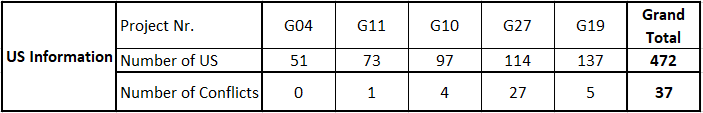
\includegraphics[scale=0.7]{Table/conflict_performance_env.png}
		\captionof{table}{Information on the backlog datasets provided for the application of the performance test}\label{tb:conflict_performance_env}
		\endgroup
	\end{figure}
	\item Tool Execution: Each part of toolchain (USPartExtractor, ActionsAnnotationsCreator, and ReportMaker) was run for each backlog and the total time taken to process the entire backlog was recorded. The performance of the tool was measured by the processing time, i.e. the total time taken to process all USs in the backlog and identify conflicts and reporting.
	
	\item Repeating Tests: To ensure reliability, each test was conducted multiple times, and the average processing time was calculated.
\end{enumerate}
The test environment consisted of:
\begin{itemize}
	\item Processor: Intel(R) Core(TM) i7-8565U CPU @ 1.80GHz (8 CPUs), ~2.0GHz		
	\item Memory: 8070MB RAM
	\item Display Devices: Intel(R) UHD Graphics 620, 4163 MB(Display Memory)
	\item Hard Disk: INTEL SSDPEKNW512G8H
	\item Operating System: Windows 11 Home 64-bit (10.0, Build 22631) (22621.ni\_release .220506-1250)
	\item System Type: 64-bit operating system, x64-based processor
\end{itemize}
Table \ref{tb:conflict_performance_result} shows the result of tool's performance in seconds which were conducted on a controlled environment to ensure consistency.
	\begin{figure}[h]
	\begingroup
	\scriptsize
	\centering
	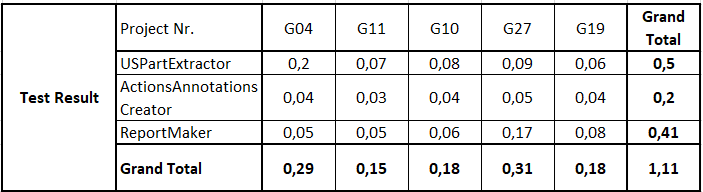
\includegraphics[scale=0.75]{Table/conflict_performance_result.png}
	\captionof{table}{Information about the result of the tool's performance test, which was measured using the processing time in seconds.}\label{tb:conflict_performance_result}
	\endgroup
\end{figure}
\paragraph{RQ2: Conclusion}There is no direct relationship between the count of USs in a backlog and the processing time required by our tool (G27 vs G19).
However, there is a direct relationship between the count of conflicts found between USs and the processing time. The more conflicts there are, the longer the processing time. 

Overall, developers and project managers with a growing backlog can expect the tool to take a reasonable amount of time to assess conflicts.
\subsubsection*{Threats to Validity}
Several potential threats to validity need to be considered when assessing the conflicts between USs both by personal judgement (ground truth) and by the automated tool. This section outlines the main threats to validity and describes how they were mitigated during the study.
\paragraph{Construct validity}It refers to how accurately the assessment measures what it is supposed to measure. The following risks have been identified:
\begin{itemize}
	\item Ambiguity of criteria: If the criteria for conflict are unclear or open to interpretation, this can lead to inconsistent scores. To avoid this, we defined clear and detailed criteria for identifying conflicts in USs.
	
	\item Ambiguity of action-annotations: If the action-annotations associated with each verb in a US are unclear or not specific to the context, this can lead to inconsistent scores. To prevent this, we assign the action-annotations based on the context of the backlog instead of using general terms.
	
	\item Subjectivity in ground truth: Since the ground truth is based on personal judgements, subjectivity could lead to bias. To minimise this risk, the evaluator (in this case me) has cross-checked the evaluations several times.
\end{itemize}
\paragraph{External validity}External validity refers to how well the results of the study can be transferred to other contexts or populations. Threats to external validity include:

\begin{itemize}
	\item specificity of USs: If the USs in the study are too specific or specific to the context, the results may not be transferable to other projects. To avoid this, we analysed 19 backlog datasets with different USs and project types.
	
	\item Tool Limitations:
	\begin{itemize}
		
	 \item The automated tool is tailored to a specific format of USs, which limits its wider applicability. It is highly dependent on the exact structure of USs (e.g. "As \textless role\textgreater I want to ..., so that ..."), which is crucial for its functionality. Therefore, we evaluated the tool in controlled environments, focussing exclusively on well-structured USs, and investigated its performance in different scenarios.
	
	\item Our tool relies on a specific type of annotations for USs, e.g. action, entity, their reference targets, triggers and contains. The effectiveness of the tool depends on these annotations being accurate and consistent. If the annotations are incomplete or incorrect, the tool may not work properly. Also, the tool may not be compatible with other annotation schemes that use different labels.
	
	\item The verbs in the action-annotation reference database are not included in their root form, but as they actually occur in the USs. This means that the same verb in different forms may be found in the database.
\end{itemize}
\end{itemize}
\paragraph{Internal Validity}Internal validity is concerned with whether the observed results are attributable to the factors analysed or are influenced by other variables. Potential threats to internal validity include:
\begin{itemize}
	\item Confounding factors: External factors or unintended variables can influence the evaluation of the conflicts analysis. In particular, the USs annotated with Doccano have a significant influence on the conflicts analysis. The more phrases are covered as label (especially as entity and action), the better the result of evaluation. Since our tool uses Doccano-annotated USs without changes as primary input, these discrepancies are unavoidable.
	
	\item Limitation of tool: The automated tool does not take into account the analysis of conflicts in the benefit parts of the USs.
\end{itemize}
\subsection{Conclusion}\label{conflict_conclustion}
In this study, we introduced an approach that integrates the Doccano tool and our custom tool to systematically identify and report conflicts between USs in software development projects. We also conducted an evaluation of this approach.

By carefully analysing 19 different backlog datasets, our method not only separated the USs into main and benefit parts for nuanced examination, but also facilitated conflicts analysis by translating the verbs of the main parts into four distinct categories, namely "delete", "create", "forbid" and "preserve", and finally reported the potential conflicts in text base format.

Our results reveal a decisive finding: the effectiveness of conflicts analysis is significantly influenced by the quality of the USs and their annotations. Well-formulated USs, in which general verbs (e.g. "have", "know") and nouns (e.g. "data", "list", "collection") are avoided, as well as a concisely annotated backlog with precise labelling of the entities (nouns) significantly improve the effectiveness of the conflicts analysis.

 If the main parts of a US-pair contradict each other, the application of one US has a negative effect on another US by deleting a resource that another US uses, or creating a resource that another US prohibits, or deleting a resource that another US also wants to delete.
 
 If conflicts between USs are identified, this is a signal for the project team to take a closer look at the requirements and the design of the system. By prioritising, sequencing, defining clear rules, implementing conflict resolution mechanisms, refining USs and involving stakeholders, the team can effectively manage and resolve these conflicts to ensure a well-functioning system.
 
In summary, our study confirms the central role of a semantic analysis approach in the detection and management of conflicts in project backlogs and thus contributes to the rationalisation of software development processes.

The quality of the annotated USs and their well-formed structure are central to the success of this approach. The results of this study provide useful guidance for improving current practices and shaping future research in software project management.

